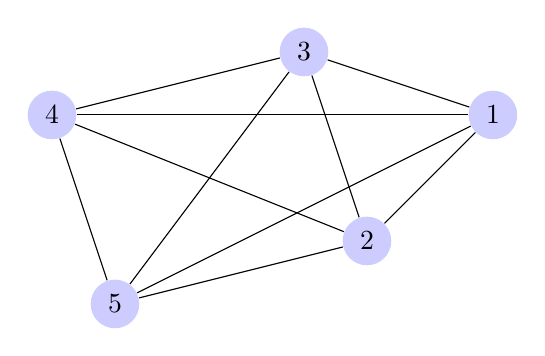
\begin{tikzpicture}
  [scale=.8,auto=left,every node/.style={circle,fill=blue!20} ]%edge/.style={bend left}]
  \node (n4) at (4,8)  {4};
  \node (n5) at (8,9)  {3};
  \node (n1) at (11,8) {1};
  \node (n2) at (9,6)  {2};
  \node (n3) at (5,5)  {5};`

  \foreach \from/\to in {n1/n2,n1/n3,n1/n4,n1/n5,n2/n3,n2/n4,n2/n5,n3/n4,n3/n5,n4/n5}
    \draw (\from) -- (\to);

\end{tikzpicture}

